
%%%%%%%%%%%%%%%%%%%%%%%%%

\section{Motivation} \label{intro:motivation}

%\subsection{Standardised uncertainty quantification tool}
%\subsection{UQ for sequence-to-sequence models}

Uncertainty quantification (UQ) methods are essential to assess the quality and performance of models and ultimately build more robust, reliable and trustworthy machine learning systems. Indeed, predictions are frequently used to make informed decisions, and the inability to understand their reliability may compromise that process. This is particularly relevant in present times since models start to interact with real-life environments along with humans around them. In industries such as healthcare or transportation, confident yet incorrect predictions could result in devastating outcomes. Consequently, trust is a fundamental ingredient for adopting real-life machine learning systems.
% statistical ML point
In addition, models are based on the concept of generalisation, i.e. the ability to perform almost as well on unseen data. This concept derives from the underlying assumption that the test set is drawn from the same statistical distribution as the training set. However, this assumption is often violated in production environments due to large occurrences of unexpected edge cases, e.g. abnormal obstacles for self-driving cars (cf. figure \ref{fig:discrepancies-train-test-distributions}).
With the rise of large language models like BERT, BLOOM, GPT3 and ChatGPT, natural-language processing and, in particular, text generation is also one of the research areas demonstrating a growing concern for uncertainty estimation. Such models often produce incorrect or misleading outputs, i.e. hallucinations, which result from different sources of uncertainty. 

Overall, uncertainty quantification is a crucial step towards reliable ML systems in academia and the industry. However, most of the existing literature is either domain or task-specific.
The lack of standardisation prevents effectively productionalising these models across a variety of applications\cite{surveyUQinDL}. In this thesis, a simple and ready-to-use toolbox is built. It follows the \textit{scikit-learn} API to train and evaluate UQ models. 

% motivation for oracle
%Oracle intends to use this tool to develop further one of its products used in the financial domain. The product includes machine learning models that produce predictions to be used by decision-makers. Indeed, they hope to be able to move away from point estimates and provide decision-makers with a tool to estimate the model's confidence or uncertainty when analysing model predictions. Besides this product, Oracle has focused on developing graph-to-text and text-graph models. They are based on sequence-to-sequence transformers such as T5. Understanding the uncertainty in these models can help identify areas where models may be prone to errors and take steps to mitigate them. 




\begin{figure}
     \centering
     \begin{subfigure}[b]{0.49\textwidth}
         \centering
         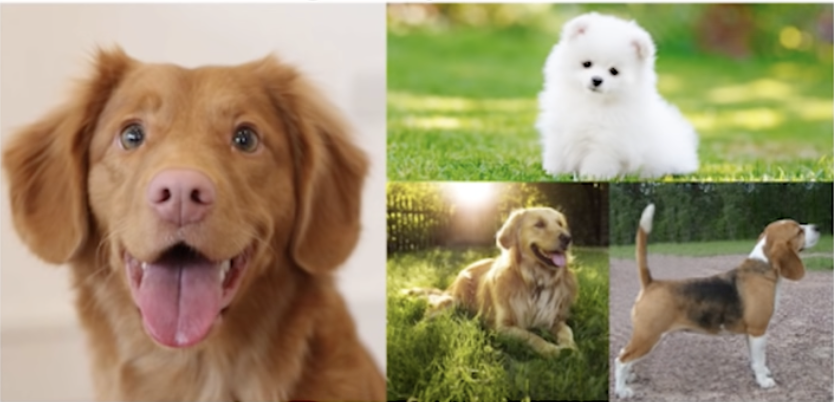
\includegraphics[width=\textwidth]{figures/intro/dogs_train.png}
         \caption{Dogs train set.}
     \end{subfigure}
     \hfill
     \begin{subfigure}[b]{0.49\textwidth}
         \centering
         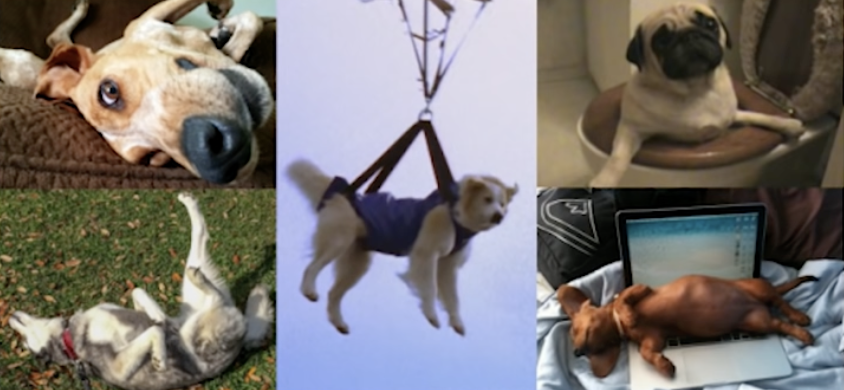
\includegraphics[width=\textwidth]{figures/intro/dogs_test.png}
         \caption{Dogs test set.}
     \end{subfigure}

     \hfill
     \begin{subfigure}[b]{0.49\textwidth}
         \centering
         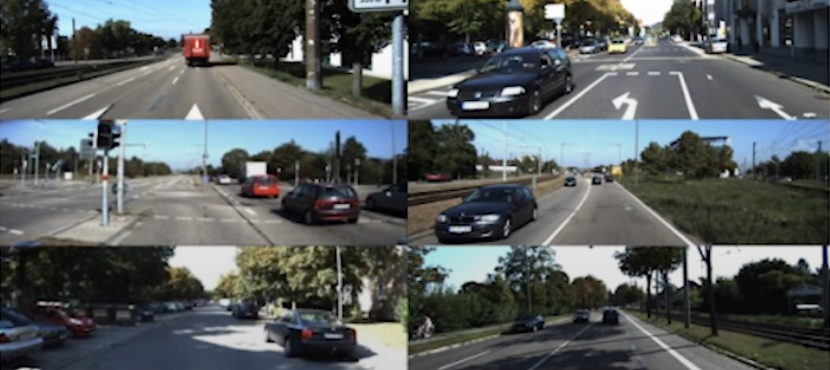
\includegraphics[width=\textwidth]{figures/intro/cars_train.png}
         \caption{Cars train set.}
     \end{subfigure}
     \hfill
     \begin{subfigure}[b]{0.49\textwidth}
         \centering
         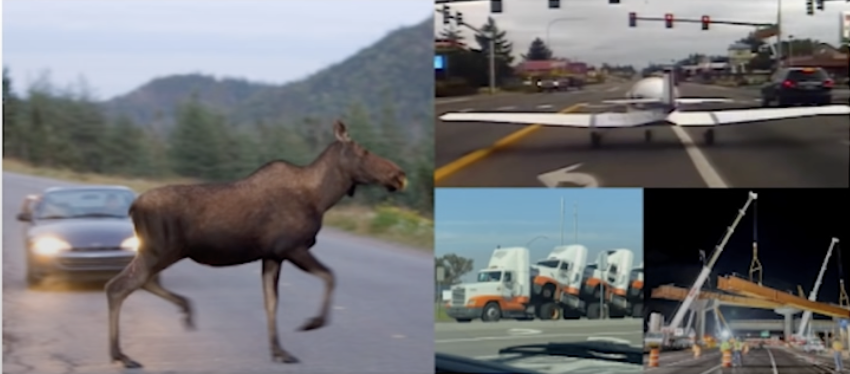
\includegraphics[width=\textwidth]{figures/intro/cars_test.png}
         \caption{Cars test set.}
     \end{subfigure}
     \caption{Discrepancies between training and testing 
     distributions (\href{http://introtodeeplearning.com/2021/slides/6S191_MIT_DeepLearning_L7.pdf}{source}).}
     \label{fig:discrepancies-train-test-distributions}
\end{figure}

\section{Objectives}

The purpose of this thesis is twofold:
\begin{enumerate}
    \item On the one hand, to build a Python package that offers a standardised \textit{scikit-learn} compatible API to train and evaluate uncertainty quantification models. This package shall be able to transform any classification or regression model following a \textit{scikit-learn} API into an updated model capable of evaluating its uncertainty.
    \item On the other hand, to provide insights into the occurrence of hallucinations in the current graph-to-text pipeline at Oracle and how they can be related to uncertainty. The following research questions shall be answered:
    \begin{enumerate}
        \item What are the different approaches to estimating uncertainty in text generation and/or sequence-to-sequence models? How do these approaches compare in terms of performance?
        \item What is the relationship between uncertainty and hallucination? To what extent is it possible to use uncertainty quantification to detect hallucinations?
    \end{enumerate}

\end{enumerate}

\section{Problem statement} \label{intro:problem-section}

%\subsubsection{The uncertainty function}

As discussed in the previous sections, understanding how much evidence the model has in its predictions can be equally as important as the predictions themselves. The quantification of uncertainty can be formalised as follows. Let $D_{train}=\{x_i\}_{i=1}^N$ be the training dataset where each data point is $D$ dimensional and let $\hat y_i = f(x_i)$ be the models predictions. The goal of UQ is to produce scores 
$u_i = U_f(x_i)$
such that $u_i$ is high when the model error is high and conversely. The usual candidates for the uncertainty function $U$ are the standard deviation (respectively the entropy) of the prediction distribution in the regression (respectively classification) case.   
Furthermore, two scenarios can occur during the evaluation on a testing data set $D_{test}$, which may not follow the same underlying distribution as $D_{train}$, i.e. out of distribution data points. On the one hand, the model may perform similarly on $D_{test}$ compared to $D_{train}$, which indicates a low generalisation error. In this case, the uncertainty should be roughly comparable between the two datasets. On the other hand, the model may under-perform on $D_{test}$ and the following property is expected to hold

\begin{equation}
    \E_{p(X \mid D_{test})} [U_f(X)] \geq  \E_{p(X \mid D_{train})} [U_f(X)] 
\end{equation}

If not, it implies that the model is more confident over incorrect predictions, which is a failure for $U$ to capture the inherent uncertainty of the model.
If this definition covers most classification use cases, it needs to be slightly adapted for text generation. Indeed, the output of the model is composed of multiple tokens 
$
\hat y_i = [t_{i,1}, \ldots, t_{i,L}]
$
and it is natural to define the uncertainty function at the same token granularity
$
u_i = [u_{i,1}, \ldots, u_{i,L}]
$.
Nevertheless, for readability purposes, these scores could be aggregated into decoded words, sentences, etc.

\section{Illustrative examples}

This section contains visual interpretations of the output of UQ models for a regression and a text generation use case.
For the first case, UQ usually consists of confidence intervals or standard deviations. In figure \ref{fig:uq-regression-example}, three different UQ model predictions are displayed for the same underlying mean prediction function. Ultimately, the objective of UQ models is to reach the performance of the third model (cf. figure \ref{uq-regression-example-calibrated}) so that it is neither over nor under-confident and these uncertainty scores can be trusted by the model's user. 

\begin{figure}
     \centering
     \begin{subfigure}[b]{0.32\textwidth}
         \centering
         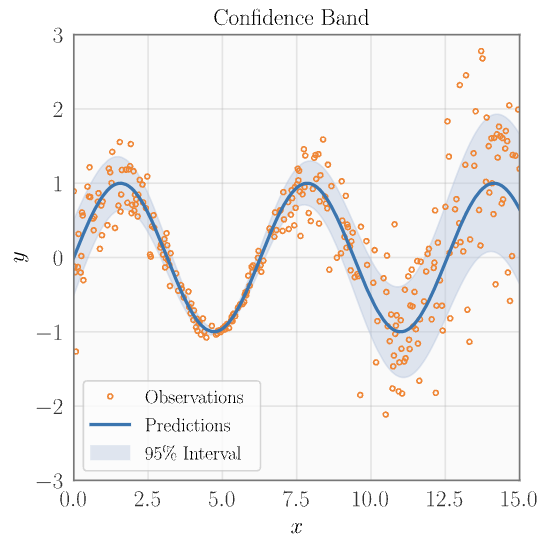
\includegraphics[width=\textwidth]{figures/intro/example-under.png}
         \caption{Over-confident UQ model.}
        % \label{fig:y equals x}
     \end{subfigure}
     \hfill
     \begin{subfigure}[b]{0.32\textwidth}
         \centering
         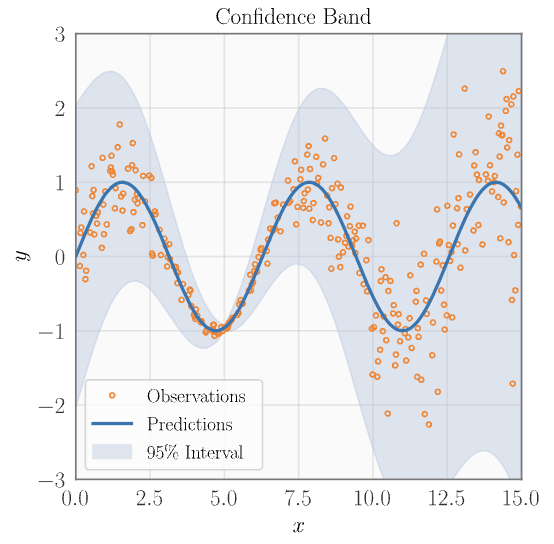
\includegraphics[width=\textwidth]{figures/intro/example-over.png}
         \caption{Under-confident UQ model.}
       %  \label{fig:three sin x}
     \end{subfigure}
     \hfill
     \begin{subfigure}[b]{0.32\textwidth}
         \centering
         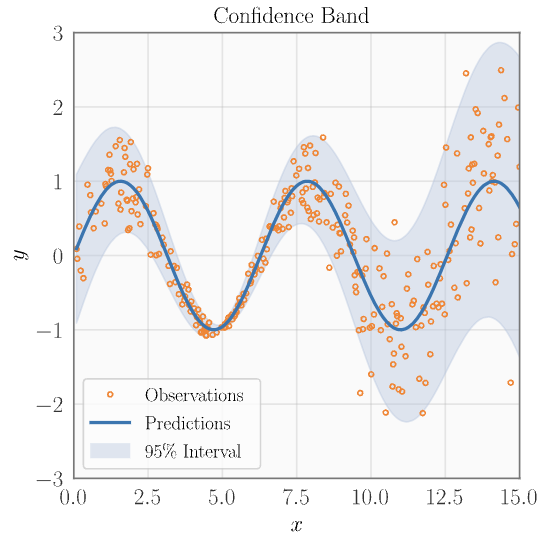
\includegraphics[width=\textwidth]{figures/intro/example-good.png}
         \caption{Calibrated UQ model.}
         \label{uq-regression-example-calibrated}
     \end{subfigure}
        \caption{Examples of uncertainty quantification models for regression (\href{https://github.com/uncertainty-toolbox/uncertainty-toolbox}{source}).}
        \label{fig:uq-regression-example}
\end{figure}

% Example: forecasting model of the return of a portfolio over time. 

When it comes to text generation, one particular text instance of the WebNLG dataset is considered, as well as the following model response, in an attempt to reproduce this text.

\epigraph{Alan Bean was an American astronaut, born on March 15, 1932, in Wheeler, Texas. He received a Bachelor of Science degree at the University of Texas at Austin in 1955 and was chosen by NASA in 1963.}{Reference text}

\epigraph{
Alan Bean was an American astronaut, born on March 15, \textbf{1948}, in Wheeler, Texas. He received a Bachelor of Science degree at the \textbf{Massachusetts Institute of Technology} in 1955 and was selected by NASA in 1963.
}{Model prediction}

The model has introduced some errors for the birth year as well as the name of the college university. A valid uncertainty quantification model should produce an output similar to the following. Note that uncertainty scores appear on top of the text with the convention that higher red intensity corresponds to a higher uncertainty score.

\epigraph{
Alan Bean was an American astronaut, born on \textcolor{Salmon}{\textbf{March}} 15, \textcolor{BrickRed}{\textbf{1948}} in Wheeler, Texas. He \textcolor{Salmon}{\textbf{received a}} Bachelor of Science degree at the \textcolor{BrickRed}{\textbf{Massachusetts Institute}}  \textcolor{Salmon}{\textbf{ of Technology}} in 1955 and was \textcolor{Salmon}{\textbf{selected}} by NASA in 1963.
}{Model prediction with uncertainty}




